\chapter{Detection: Board A}
\label{cap:detection}

La Board A è responsabile del primo stadio della pipeline ALPR: a partire da un'immagine 192$\times$192 grayscale ricevuta dal PC, deve individuare la regione contenente la targa, ritagliarla e inoltrarla alla Board B per il riconoscimento dei caratteri. Questo capitolo descrive la rete neurale impiegata, il processo di addestramento, la validazione, l'esportazione del modello e l'implementazione del firmware Zephyr che lo integra.

\section{Rete YOLOv8-tiny custom}
\label{sec:yolov8t}

La rete utilizzata è una variante personalizzata di YOLOv8, ridotta in scala per adattarsi ai vincoli di memoria del microcontrollore. Il framework Ultralytics non prevede ufficialmente una scala più piccola della \texttt{n} (\textit{nano}); è stata quindi definita manualmente una nuova scala denominata \texttt{t} (\textit{tiny}), caratterizzata da un fattore di larghezza dei canali pari a $0{,}125$, esattamente la metà di quello di YOLOv8n, e da una profondità di $0{,}33$. Il file di configurazione della rete è stato inoltre modificato per accettare in ingresso immagini a singolo canale (\texttt{ch:~1}) e prevedere una singola classe (\texttt{nc:~1}), corrispondente all'etichetta \texttt{license\_plate}. La porzione rilevante del file di configurazione è riportata nel Listing~\ref{lst:yolo-yaml}.

\begin{lstlisting}[style=stileYAML, caption={Configurazione \texttt{yolov8t.yaml} che definisce la scala \texttt{t} a singolo canale e singola classe.}, label={lst:yolo-yaml}]
ch: 1
nc: 1
scales:
  t: [0.33, 0.125, 512]  # tiny: width 0.125 = meta di yolov8n


backbone:
  - [-1, 1, Conv, [64, 3, 2]]
  - [-1, 1, Conv, [128, 3, 2]]
  - [-1, 3, C2f, [128, True]]
  - [-1, 1, Conv, [256, 3, 2]]
  - [-1, 6, C2f, [256, True]]
  - [-1, 1, Conv, [512, 3, 2]]
  - [-1, 6, C2f, [512, True]]
  - [-1, 1, Conv, [1024, 3, 2]]
  - [-1, 3, C2f, [1024, True]]
  - [-1, 1, SPPF, [1024, 5]]

head:
  - [-1, 1, nn.Upsample, [None, 2, "nearest"]]
  - [[-1, 6], 1, Concat, [1]]
  - [-1, 3, C2f, [512]]
  - [-1, 1, nn.Upsample, [None, 2, "nearest"]]
  - [[-1, 4], 1, Concat, [1]]
  - ...
\end{lstlisting}

\section{Addestramento}
\label{sec:addestramento}

L'intero processo di addestramento è stato sviluppato su Google Colab utilizzando il framework Ultralytics, a partire dal dataset open source \textit{License-Plate-Recognition} (versione 4) pubblicato sulla piattaforma Roboflow Universe~\cite{roboflow_universe}. Il dataset contiene immagini di veicoli a colori con annotazioni dei bounding box delle targhe in formato YOLO, suddivise nei tre split di training, validation e test secondo la ripartizione predefinita dal pubblicatore.

\subsection{Preparazione del dataset}
\label{sec:dataset-prep}

Poiché la rete è progettata per accettare in ingresso immagini a singolo canale, è stato implementato uno script Python che converte in scala di grigi tutte le immagini dei tre split e aggiorna il file di configurazione \texttt{data.yaml} aggiungendo il parametro \texttt{channels:~1}, necessario per istruire Ultralytics sulla natura monocromatica dei dati. La conversione è parallelizzata su otto thread tramite \texttt{ThreadPoolExecutor} e gestisce in modo robusto eventuali file corrotti, rimuovendoli insieme alle relative etichette per non compromettere l'integrità del training.

\begin{lstlisting}[style=stilePython, caption={Conversione del dataset in scala di grigi.}, label={lst:gray-conversion}]
def converti_singola(img_path):
    try:
        img = Image.open(img_path).convert("L")
        img.save(img_path)
    except Exception:
        corrotte.append(img_path)
        img_path.unlink()

def converti_grayscale(dataset_path):
    for split in ["train", "valid", "test"]:
        img_dir = Path(dataset_path) / split / "images"
        images = list(img_dir.glob("*.jpg")) + \
                 list(img_dir.glob("*.jpeg")) + \
                 list(img_dir.glob("*.png"))
        with ThreadPoolExecutor(max_workers=8) as executor:
            executor.map(converti_singola, images)

# Aggiunta del campo channels nel data.yaml
data_info['channels'] = 1
\end{lstlisting}

\subsection{Configurazione e training}
\label{sec:train-config}

Il file di configurazione della rete è ottenuto a partire dal \texttt{yolov8.yaml} ufficiale di Ultralytics, modificato per introdurre la scala personalizzata \texttt{t} (\textit{tiny}) e per dichiarare il singolo canale in input e la singola classe in output. Una volta scritto su disco il file modificato, il modello viene istanziato direttamente dal file YAML senza partire da pesi pre-addestrati, perché la modifica del numero di canali in ingresso renderebbe incompatibili i pesi standard distribuiti per la versione RGB. L'addestramento è eseguito tramite il metodo \texttt{train()} dell'oggetto \texttt{YOLO}, con i parametri riportati sotto. I valori più significativi sono \texttt{epochs=50} (numero massimo di epoche), \texttt{patience=15} (\textit{early stopping} dopo 15 epoche senza miglioramenti), \texttt{imgsz=192} (risoluzione di ingresso fissata), \texttt{batch=64} (dimensione del batch), \texttt{lr0=0.01} (learning rate iniziale) e \texttt{pretrained=False} (training da zero per i motivi appena spiegati).

\begin{lstlisting}[style=stilePython, caption={Avvio dell'addestramento della rete YOLOv8-tiny custom.}, label={lst:training}]
model = YOLO(yaml_path)

results = model.train(
    data=f"{dataset.location}/data.yaml",
    epochs=50,
    imgsz=192,
    batch=64,
    patience=15,
    device=0,
    name="yolov8t_lp_gray",
    lr0=0.01,
    pretrained=False,
)
\end{lstlisting}

\subsection{Metriche di validazione}
\label{sec:metriche}

Al termine del training, il modello con i pesi migliori (\texttt{best.pt}) viene valutato sul set di validazione attraverso il metodo \texttt{val()} di Ultralytics. Le metriche ottenute sono riportate in Tabella~\ref{tab:yolo-metrics}. Il valore di mAP@0.5 di $0{,}941$ indica un'accuratezza elevata nel rilevamento delle targhe; il fatto che la precisione sia superiore al recall ($0{,}979$ contro $0{,}908$) suggerisce che la rete è leggermente conservativa, preferendo non emettere una detection piuttosto che produrre un falso positivo. Questo comportamento è preferibile nel contesto applicativo: una falsa detection inviata alla pipeline OCR genererebbe una stringa di output priva di significato, mentre l'assenza di detection produce una risposta esplicita di tipo \texttt{TYPE\_NONE} che l'utente sa interpretare.

\begin{table}[H]
    \centering
    \caption{Metriche di validazione del modello YOLOv8-tiny custom.}
    \label{tab:yolo-metrics}
    \begin{tabular}{lc}
        \toprule
        \textbf{Metrica} & \textbf{Valore} \\
        \midrule
        mAP@0.5         & $0{,}941$ \\
        mAP@0.5:0.95    & $0{,}638$ \\
        Precision       & $0{,}979$ \\
        Recall          & $0{,}908$ \\
        F1 score        & $0{,}942$ \\
        \bottomrule
    \end{tabular}
\end{table}

\section{Test della rete addestrata}
\label{sec:testing-rete}

La fase di test è stata eseguita ancora nell'ambiente Colab, sfruttando l'API di Ultralytics, per verificare in modo qualitativo il comportamento del modello prima di affrontare la quantizzazione INT8 e l'esecuzione embedded. Le immagini di test sono state pre-elaborate con la stessa procedura applicata al dataset di training: conversione in scala di grigi tramite il metodo \texttt{convert("L")} di PIL e mantenimento del formato originale. La fase di inferenza è effettuata invocando il metodo \texttt{predict()} del modello, passando il percorso della cartella contenente le immagini di test, una soglia di confidenza di $0{,}5$ e la stessa risoluzione di $192\times192$ utilizzata in addestramento (Listing~\ref{lst:predict}).

\begin{lstlisting}[style=stilePython, caption={Inferenza su un insieme di immagini di test tramite l'API Ultralytics.}, label={lst:predict}]
best_model = YOLO("runs/detect/yolov8t_lp_gray/weights/best.pt")

results = best_model.predict(
    source=str(test_dir),
    conf=0.5,
    imgsz=192,
    save=False,
    verbose=False
)

# Estrazione di statistiche per ciascuna immagine
for result in results:
    n_plates = len(result.boxes)
    for box in result.boxes:
        conf = box.conf.item()
        xyxy = box.xyxy[0].tolist()
        # ...
\end{lstlisting}

Per ciascuna immagine processata vengono estratte le coordinate del bounding box e il valore di confidenza associato, e l'immagine viene visualizzata con il rettangolo della detection sovrapposto attraverso il metodo \texttt{plot()} fornito da Ultralytics. La Figura~\ref{fig:test-results} mostra una selezione dei risultati ottenuti su un campione di immagini di test contenenti targhe di paesi diversi.

\begin{figure}[H]
    \centering
    \begin{subfigure}[t]{0.48\textwidth}
        \centering
        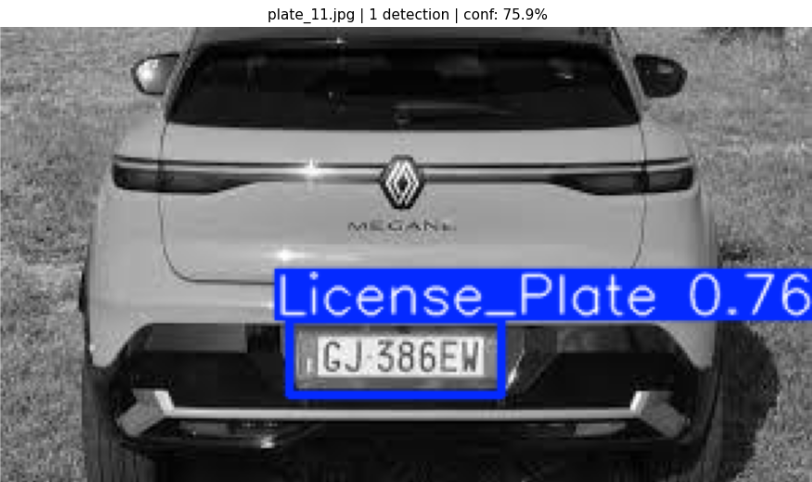
\includegraphics[width=0.80\textwidth]{images/yolov8t_test/plate_a.png}
        \label{fig:test-a}
    \end{subfigure}
    \hfill
    \begin{subfigure}[t]{0.48\textwidth}
        \centering
        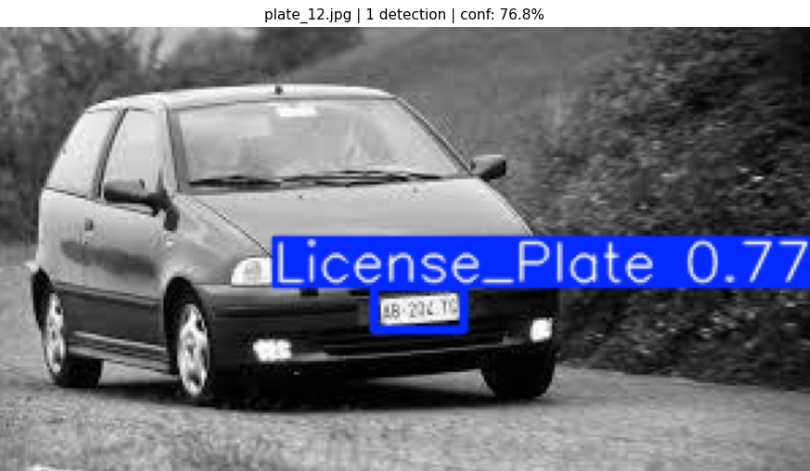
\includegraphics[width=0.80\textwidth]{images/yolov8t_test/plate_b.png}
        \label{fig:test-b}
    \end{subfigure}

    \vspace{0.4em}

    \begin{subfigure}[t]{0.48\textwidth}
        \centering
        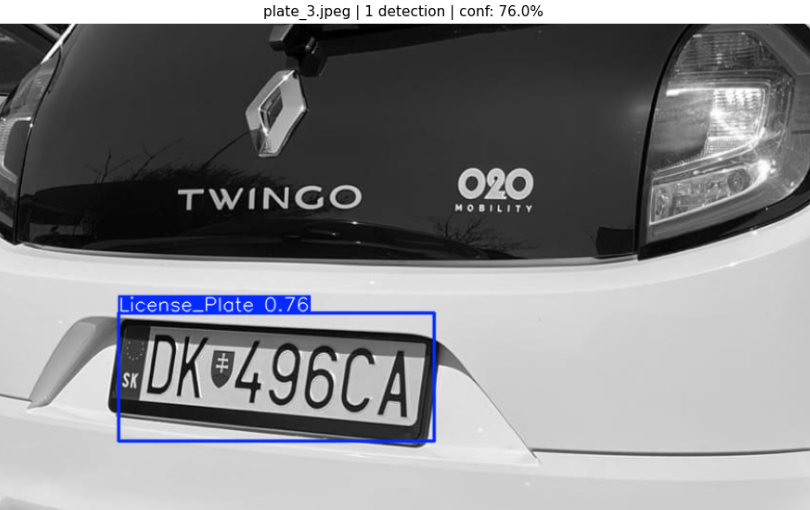
\includegraphics[width=0.80\textwidth]{images/yolov8t_test/plate_c.png}
        \label{fig:test-c}
    \end{subfigure}
    \hfill
    \begin{subfigure}[t]{0.48\textwidth}
        \centering
        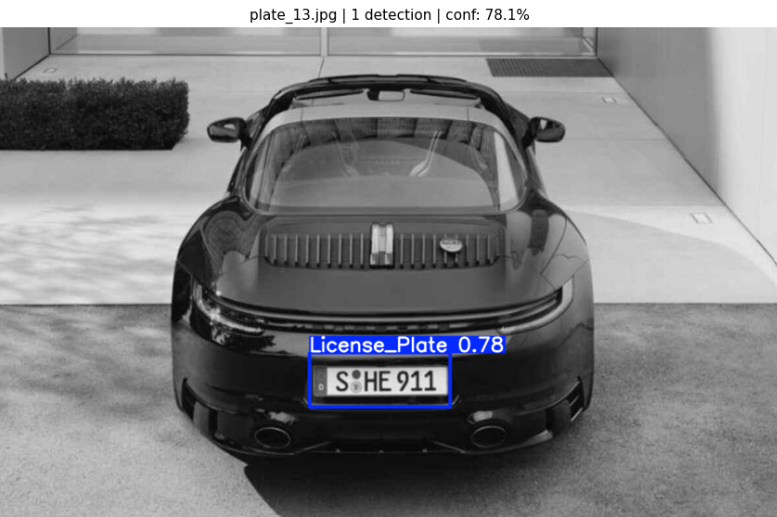
\includegraphics[width=0.80\textwidth]{images/yolov8t_test/plate_d.png}
        \label{fig:test-d}
    \end{subfigure}

    \caption{Esempi di output del modello YOLOv8-tiny custom su immagini di test.}
    \label{fig:test-results}
\end{figure}

I risultati di questa validazione preliminare hanno confermato che il modello generalizza correttamente su immagini esterne al dataset di addestramento, con confidenze tipicamente comprese tra $0{,}66$ e $0{,}96$ e un singolo caso di mancata detection in corrispondenza di un'immagine che non conteneva alcun veicolo.


%==============================================

\section{Esportazione ONNX e quantizzazione con X-CUBE-AI}
\label{sec:onnx-split}
 
Conclusa la fase di addestramento e validazione su Colab, il modello viene portato sul microcontrollore attraverso un processo a due passi: prima l'esportazione del file \texttt{best.pt} di Ultralytics in formato ONNX, poi l'importazione del file ONNX nello strumento X-CUBE-AI di STMicroelectronics che si occupa di quantizzare i pesi a INT8 e di generare la libreria C statica da linkare al firmware.
 
\subsection{Esportazione con output splittati}
\label{sec:export-split}
 
L'esportazione viene effettuata tramite l'API \texttt{export()} di Ultralytics con risoluzione di ingresso fissata a 192 e l'opzione \texttt{simplify=True}, che rimuove dal grafo i nodi ridondanti o di identità prodotti durante la conversione e ne agevola l'importazione in X-CUBE-AI. L'esportazione standard produce però un grafo che termina con un nodo \texttt{Concat} che combina i bounding box e le confidenze in un unico tensore di output di forma $[1, 5, 756]$. Questa rappresentazione è scomoda per il passo di quantizzazione successivo, perché i due flussi hanno intervalli di valori molto diversi: i bounding box assumono valori nell'intervallo $[0, 192]$ in coordinate pixel, mentre le confidenze sono limitate a $[0, 1]$. Forzare entrambi nello stesso tensore quantizzato in INT8 con un unico \textit{scale} comporterebbe una notevole perdita di precisione sulle confidenze, che si schiaccerebbero su pochi livelli di quantizzazione. Per questo motivo il nodo \texttt{Concat} finale è stato rimosso manipolando direttamente il grafo ONNX con la libreria \texttt{onnx}, e i due tensori intermedi (\texttt{boxes}, di forma $[1, 4, 756]$, e \texttt{conf}, di forma $[1, 1, 756]$) sono stati resi come output indipendenti. In questo modo X-CUBE-AI quantizza i due tensori con \textit{scale} e \textit{zero-point} separati, preservando la precisione di entrambi.
 
\subsection{Importazione in X-CUBE-AI}
\label{sec:cube-import}
 
X-CUBE-AI è il pacchetto di STMicroelectronics che importa modelli di reti neurali in formato ONNX, ne effettua la quantizzazione e ne genera una libreria C ottimizzata per la famiglia STM32 target. Il flusso di import è il medesimo per i due modelli del progetto e si articola in tre fasi:
 
\begin{enumerate}
    \item \textbf{Caricamento del modello}: il file ONNX viene importato nello strumento, che ne mostra le caratteristiche essenziali (dimensione dell'input, formato degli output, tipo dei dati).
    \item \textbf{Post-training quantization}: il flusso di quantizzazione è basato su ONNX Runtime e supporta sia una modalità con calibration dataset (un piccolo insieme di campioni in formato \texttt{.npz} che viene usato per stimare gli intervalli dinamici di pesi e attivazioni) sia una modalità con valori casuali, in cui gli intervalli vengono dedotti automaticamente. Nel progetto è stata scelta la modalità con valori casuali, accettando un'eventuale piccola degradazione di accuratezza in cambio di un flusso di lavoro più semplice e replicabile.
    \item \textbf{Ottimizzazione e generazione della libreria}: lo strumento offre tre profili di ottimizzazione:\textit{balanced}, \textit{RAM} e \textit{time}. Considerati i vincoli stringenti di memoria della STM32H745, è stato selezionato per entrambi i modelli il profilo \textit{optimization=ram}, che minimizza la dimensione dell'\textit{activation buffer} a scapito di un possibile leggero aumento del tempo di inferenza.
\end{enumerate}
 
\subsection{Risultati dell'ottimizzazione}
\label{sec:cube-results}
 
Al termine del passo di ottimizzazione, sul tool viene riportata una tabella riassuntiva con il numero di operazioni necessarie per una singola inferenza (MACC, \textit{Multiply-Accumulate operations}), l'occupazione di Flash distinta tra pesi e libreria runtime, e l'occupazione di RAM distinta tra \textit{activation buffer} e contesto della libreria. La Figura~\ref{fig:cube-stats} mostra l'output ottenuto per i due modelli e la Tabella~\ref{tab:cube-stats} ne riassume i numeri.
 
\begin{figure}[H]
    \centering
    \begin{subfigure}[t]{\textwidth}
        \centering
        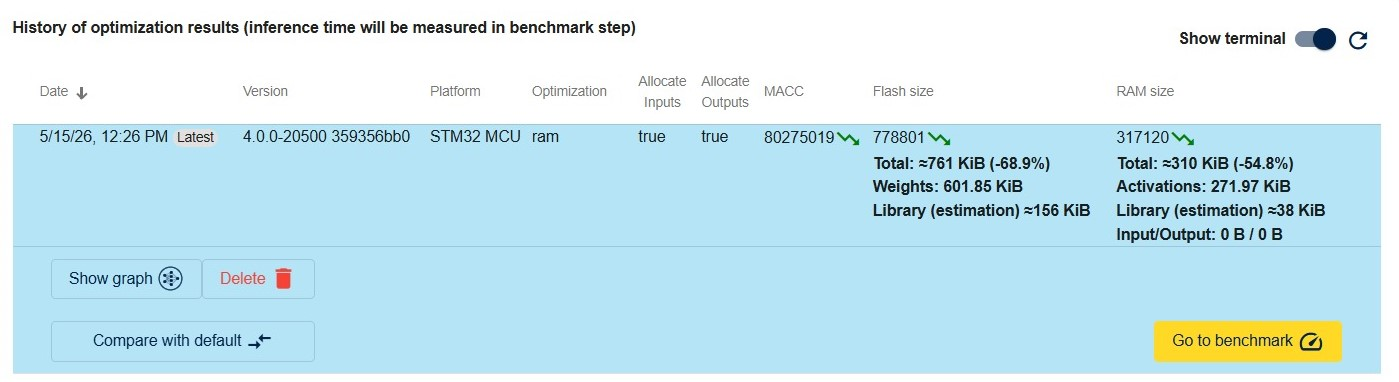
\includegraphics[width=0.90\textwidth]{images/xcubeai/xcubeai_a.jpeg}
        \caption{Risultati dell'ottimizzazione del detector YOLO con profilo \textit{ram}.}
        \label{fig:opt-yolo}
    \end{subfigure}
 
    \vspace{0.5em}
 
    \begin{subfigure}[t]{\textwidth}
        \centering
        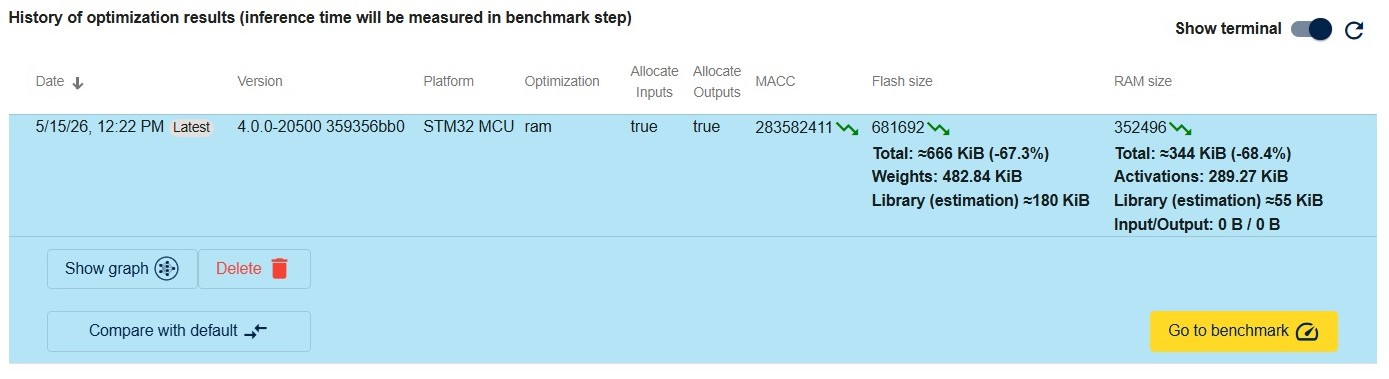
\includegraphics[width=0.90\textwidth]{images/xcubeai/xcubeai_b.jpeg}
        \caption{Risultati dell'ottimizzazione dell'OCR CCT-XS con profilo \textit{ram}.}
        \label{fig:opt-cct}
    \end{subfigure}
    \caption{Output di X-CUBE-AI al termine del passo di ottimizzazione per i due modelli.}
    \label{fig:cube-stats}
\end{figure}
 
\begin{table}[H]
    \centering
    \caption{Stima di occupazione di memoria e di operazioni prodotta da X-CUBE-AI per i due modelli quantizzati con profilo \textit{optimization=ram}.}
    \label{tab:cube-stats}
    \begin{tabular}{lrr}
        \toprule
        \textbf{Voce} & \textbf{YOLOv8-tiny} & \textbf{CCT-XS} \\
        \midrule
        MACC (per inferenza)             & 80\,275\,019 & 283\,582\,411 \\
        Flash totale stimata             & $\sim$761~KiB & $\sim$666~KiB \\
        \hspace{1em}Pesi                 & 601{,}85~KiB & 482{,}84~KiB \\
        \hspace{1em}Libreria runtime     & $\sim$156~KiB & $\sim$180~KiB \\
        RAM totale stimata               & $\sim$310~KiB & $\sim$344~KiB \\
        \hspace{1em}Activation buffer    & 271{,}97~KiB & 289{,}27~KiB \\
        \hspace{1em}Libreria runtime     & $\sim$38~KiB & $\sim$55~KiB \\
        \bottomrule
    \end{tabular}
\end{table}
 
%==============================================

\section{Integrazione nel firmware}
\label{sec:firmware-A}

Il firmware della Board A è organizzato come un singolo thread principale che esegue ciclicamente le fasi di ricezione, inferenza e invio. Le strutture dati allocate staticamente sono progettate per minimizzare l'occupazione di RAM e sono riassunte in Tabella~\ref{tab:buffer-A}.

\begin{table}[H]
    \centering
    \caption{Allocazione statica della RAM nel firmware di Board A.}
    \label{tab:buffer-A}
    \begin{tabular}{lrl}
        \toprule
        \textbf{Buffer} & \textbf{Dimensione} & \textbf{Funzione} \\
        \midrule
        \texttt{io\_buf} (union)   & 36\,864 B   & Immagine in input e tensore quantizzato \\
        \texttt{act\_buf}          & 410\,112 B  & Attivazioni intermedie della rete \\
        \texttt{out\_boxes}        & 3\,024 B    & Output: $4 \times 756$ INT8 \\
        \texttt{out\_conf}         & 756 B       & Output: $1 \times 756$ INT8 \\
        \texttt{net\_ctx}          & --          & Contesto della libreria X-CUBE-AI \\
        \texttt{crop\_buf}         & 8\,196 B    & Crop $128 \times 64$ + header \\
        \texttt{rx\_rb\_pc}        & 8\,192 B    & Ring buffer UART verso PC \\
        \texttt{rx\_rb\_b2b}       & 256 B       & Ring buffer UART verso Board B \\
        \bottomrule
    \end{tabular}
\end{table}

La scelta più importante in termini di occupazione di RAM è l'uso di una \texttt{\textbf{union}} per condividere fisicamente la stessa regione di memoria tra l'immagine ricevuta dal PC e l'input quantizzato della rete. Come mostrato nel Listing~\ref{lst:union-A}, i due membri della union (\texttt{gray} a 8 bit unsigned e \texttt{net\_in} a 8 bit signed) hanno la stessa dimensione e non vengono mai usati simultaneamente: l'immagine viene prima ricevuta nella forma a 8 bit unsigned, poi convertita in-place in INT8 sottraendo $128$ a ogni pixel.

\begin{lstlisting}[style=stileC, caption={Union per la condivisione del buffer di ingresso tra l'immagine ricevuta e il tensore quantizzato. Risparmia $36\,864$ byte di RAM.}, label={lst:union-A}]
static union {
    uint8_t gray[GRAY_SIZE];
    int8_t  net_in[STAI_NETWORK_IN_1_SIZE];
} io_buf __attribute__((aligned(4)));
\end{lstlisting}



\subsection{Quantizzazione in-place}
\label{sec:quant-A}

La quantizzazione viene effettuata con un semplice ciclo che traduce ogni pixel dal range $[0, 255]$ di tipo \texttt{uint8\_t} al range $[-128, 127]$ di tipo \texttt{int8\_t}, sottraendo $128$. Lo \textit{zero-point} è quindi pari a $128$ e la \textit{scale} è $1{,}0$: la rete è stata calibrata in modo da accettare direttamente i pixel grezzi, senza ulteriori normalizzazioni.

\begin{lstlisting}[style=stileC, caption={Quantizzazione.}, label={lst:quantization}]
// Quantizzazione
for (int i = 0; i < STAI_NETWORK_IN_1_SIZE; i++)
    io_buf.net_in[i] = (int8_t)((int)io_buf.gray[i] - 128);
\end{lstlisting}

\subsection{Parsing dell'output e NMS}
\label{sec:nms-A}

Dopo l'inferenza, gli output della rete vengono dequantizzati con la formula $r = (q - z) \cdot s$, usando i parametri \texttt{scale} e \texttt{zero\_point} generati da X-CUBE-AI. La routine \texttt{parse\_output} analizza le $756$ anchor, conserva solo le candidate con confidenza superiore a $0{,}5$ e seleziona quella con confidenza massima. Su queste candidate viene poi applicata una NMS semplificata: le detection con IoU superiore a $0{,}5$ rispetto alla migliore vengono scartate. Poiché il caso d'uso prevede al massimo una targa per immagine, il risultato finale coincide normalmente con il bounding box più affidabile, mantenendo comunque una maggiore robustezza in presenza di più rilevamenti.

\subsection{Costruzione del crop}
\label{sec:crop}

Prima del ritaglio il firmware ripristina i pixel originali sommando $128$ a
ciascun byte INT8 (operazione inversa della quantizzazione), poiché la
\texttt{union} \texttt{io\_buf} è stata sovrascritta in-place durante
l'inferenza. Il bounding box viene poi espanso di 5 pixel su ogni lato e
le coordinate sono clampate ai bordi dell'immagine per evitare accessi
fuori buffer. La regione risultante è ridimensionata a $128\times64$~pixel
con interpolazione \textit{nearest-neighbor}\footnote{L'interpolazione \textit{nearest-neighbor} (o \textit{nearest neighbour}) è una tecnica di ridimensionamento delle immagini in cui ogni nuovo pixel assume il valore del pixel originale più vicino. Il metodo non introduce operazioni di media o filtraggio ed è quindi particolarmente efficiente dal punto di vista computazionale.} e inviata alla Board B come frame
\texttt{TYPE\_CROP} preceduto da un header di 4 byte con le dimensioni.

\begin{figure}[H]
    \centering
    \begin{tikzpicture}[
        font=\footnotesize,
        % --- stile dei blocchi RAM ---
        ram/.style={
            draw, thick, minimum height=0.9cm, minimum width=8cm,
            align=center, font=\small
        },
        gray_box/.style={ram, fill=custom_lightgray},
        int8_box/.style={ram, fill=custom_lightblue},
        % --- stile delle frecce di transizione ---
        trans/.style={->, >=stealth, very thick, custom_blue},
        % --- etichetta laterale ---
        sidelbl/.style={font=\scriptsize\itshape, custom_gray, anchor=west},
        timelbl/.style={font=\scriptsize\bfseries, custom_red, anchor=east}
    ]

    % =================================================================
    % (a) Tre stati della stessa zona di RAM
    % =================================================================

    % --- Stato 1: dopo ricezione UART ---
    \node[timelbl] (t1) at (-0.3, 0)  {t = 1};
    \node[gray_box, right=0.1cm of t1] (s1) {
        \texttt{io\_buf.gray[]} \;--\; \texttt{uint8\_t} \;--\; pixel $\in [0, 255]$
    };
    \node[sidelbl, right=0.2cm of s1] {dopo ricezione UART};

    % --- Stato 2: dopo quantizzazione ---
    \node[timelbl, below=1.1cm of t1] (t2) {t = 2};
    \node[int8_box, right=0.1cm of t2] (s2) {
        \texttt{io\_buf.net\_in[]} \;--\; \texttt{int8\_t} \;--\; pixel $\in [-128, 127]$
    };
    \node[sidelbl, right=0.2cm of s2] {input quantizzato alla rete};

    % --- Stato 3: dopo inferenza, riconvertita ---
    \node[timelbl, below=1.1cm of t2] (t3) {t = 3};
    \node[gray_box, right=0.1cm of t3] (s3) {
        \texttt{io\_buf.gray[]} \;--\; \texttt{uint8\_t} \;--\; pixel $\in [0, 255]$
    };
    \node[sidelbl, right=0.2cm of s3] {pronto per il crop};

    % --- Frecce di transizione tra i 3 stati ---
    \draw[trans] (s1) -- node[right, font=\scriptsize, custom_blue, align=left]
        {\textbf{quantizzazione}\\$q = g - 128$} (s2);
    \draw[trans] (s2) -- node[right, font=\scriptsize, custom_blue, align=left]
        {\textbf{inferenza + dequant inversa}\\$g = q + 128$} (s3);

    % --- Annotazione "stesso indirizzo di memoria" sul lato sinistro ---
    \draw[thick, custom_red, decorate,
          decoration={brace, amplitude=6pt, mirror}]
        ($(t1.north west)+(-0.1, 0.1)$) -- ($(t3.south west)+(-0.1, -0.1)$);
    \node[custom_red, font=\scriptsize\bfseries, rotate=90, anchor=south]
        at ($(t2.west)+(-0.7, 0)$) {stessa zona di RAM (36\,864 B)};

    % =================================================================
    % (b) Confronto barra RAM: con union vs senza
    % =================================================================

    \node[font=\small\bfseries, below=1cm of s3, anchor=north]
        (label_bar) {Risparmio di RAM};

    % Posizione di partenza barre
    \coordinate (bar_origin) at ($(label_bar.south)+(0, -0.5)$);

    % --- Barra "Senza union" (2 buffer separati = 73 728 B) ---
    \node[anchor=east, font=\scriptsize] at ($(bar_origin)+(-3.6, 0)$)
        {Senza \texttt{union}:};
    \fill[custom_orange] ($(bar_origin)+(-3.5, -0.25)$)
        rectangle ($(bar_origin)+(3.5, 0.25)$);
    \node[font=\scriptsize, white, anchor=center]
        at ($(bar_origin)+(0, 0)$) {\textbf{73\,728 B} (gray + net\_in)};

    % --- Barra "Con union" (1 buffer = 36 864 B) ---
    \node[anchor=east, font=\scriptsize] at ($(bar_origin)+(-3.6, -0.8)$)
        {Con \texttt{union}:};
    \fill[custom_green] ($(bar_origin)+(-3.5, -1.05)$)
        rectangle ($(bar_origin)+(0, -0.55)$);
    \node[font=\scriptsize, white, anchor=center]
        at ($(bar_origin)+(-1.75, -0.8)$) {\textbf{36\,864 B}};

    \end{tikzpicture}

    \caption{Funzionamento della \texttt{union} nel firmware di Board A.}
    \label{fig:union-memoria}
\end{figure}